\documentclass{article}
\usepackage[utf8]{inputenc}
\usepackage[margin= 2.5cm]{geometry}
\usepackage{xcolor}
\usepackage{wrapfig}
\usepackage{graphicx}
\usepackage{hyperref}
\usepackage{subcaption}
\usepackage{float}


\title{Sports Match Outcome Prediction with Spatio-Temporal Graph Representation Learning }
%\author{Anyone}
\author{Abdolreza Mirzaei\\
        Simon Fraser University \\
        abdolreza\_mirzaei@sfu.ca 
        \and Oliver Schulte\\
        Simon Fraser University \\oschulte@cs.sfu.ca \and
        Mohammad Bahrami\\
        Isfahan University of Tech.\\
        mohammadbahrami@ec.iut.ac.ir \and
        Masoud Mousavi\\
        Isfahan University of Tech.\\
        mmousavi@ec.iut.ac.ir}
        \date{}

\begin{document}

\maketitle

\begin{abstract}
Predicting the outcome of a sport match is a widely studied challenging problem of interest to many stakeholders (media, teams, fans, bookmakers). This paper develops a novel approach to match outcome prediction that leverages graph representation learning to model team-team and team-player interactions. Both teams and players correspond to nodes in a Spatio-Temporal graph. Node embeddings capture how team/player characteristics jointly influence match outcomes.
Empirical results on a dataset of nine different football leagues demonstrate the superior performance of our graph representation approach. 
\end{abstract}

\paragraph{Problem Definition}
Basically, sports match prediction refers to predicting future outcomes based on past results and features. So in general any observation will include the information of the  two teams playing at a certain time and the result of that match. There are two different types of match predictions: {\em pre-match} and {\em live (ongoing)} prediction. In this paper, predictions are made pre-game. 
The main purpose of this paper is to predict the outcome of sports matches to \{win, lose, draw\} by just using dynamic graph (specifically Spatio-Temporal graph) representation learning and without using any hand-crafted or sport-specific features.
Another key contribution of this paper is the use of lineup information. 


\paragraph{Related Work} 

In recent years, there has been much research on the use of machine learning in the prediction of match outcomes.
These studies have mainly been based on feature engineering and have considered only a small number of leagues. Various machine learning methods including Neural Networks have been used in this field~\cite{hucaljuk2011predicting}\cite{tax2015predicting}\cite{prasetio2016predicting}\cite{constantinou2019dolores}\cite{berrar2019incorporating}\cite{hubavcek2019learning}. 
Recently, deep neural networks have been used in a few studies~\cite{danisik2018football}\cite{nyquist2017football}\cite{Pereverzeva2021PredictingSM}, and to the best of our knowledge, graph neural networks have been used in only one case~\cite{Pereverzeva2021PredictingSM}.
The majority of past research has focused on learning about teams, not players. In other words, players’ strength and lineup information, has not been considered in most previous works, despite their significant impact on match outcome prediction. 
\paragraph{Methodology}

In competitive team sports, the outcome can depend on complex interactions between opposing teams and interactions among players.
Given that at a given time t, players, teams and their relations can be expressed by a spatial graph structure and the relationships between teams/players at different times can be expressed by a temporal structure, we propose a novel framework to predict match outcome leveraging {\em Spatio-Temporal graph representation learning}. 

In the proposed Spatio-Temporal graph, each player and each team at a given time is assigned a node. An edge between teams represents a match outcome (e.g., the winner), and an edge between a team and a player represents a player appearing for a team. In more detail, at each time step, players who have played for a team are connected to it via a {\em PlayedFor} link. 
At each time step, based on the result of every match, the two competing teams nodes are connected with links of type {\em won} or {\em lost}, or {\em tied}. 
Every team or player node at time $t$ is connected to its corresponding node at time $t-1$ with the link of type {\em IsAfter}. 
These {\em IsAfter} links works as regularizers to enforce similarity between corresponding nodes at different times and also encode the players and teams evolutions.
It should be noted that for every relation its inverse relation is also used with the with opposite directionality.

\begin{wrapfigure}{r}{0.50\textwidth}
\centering
     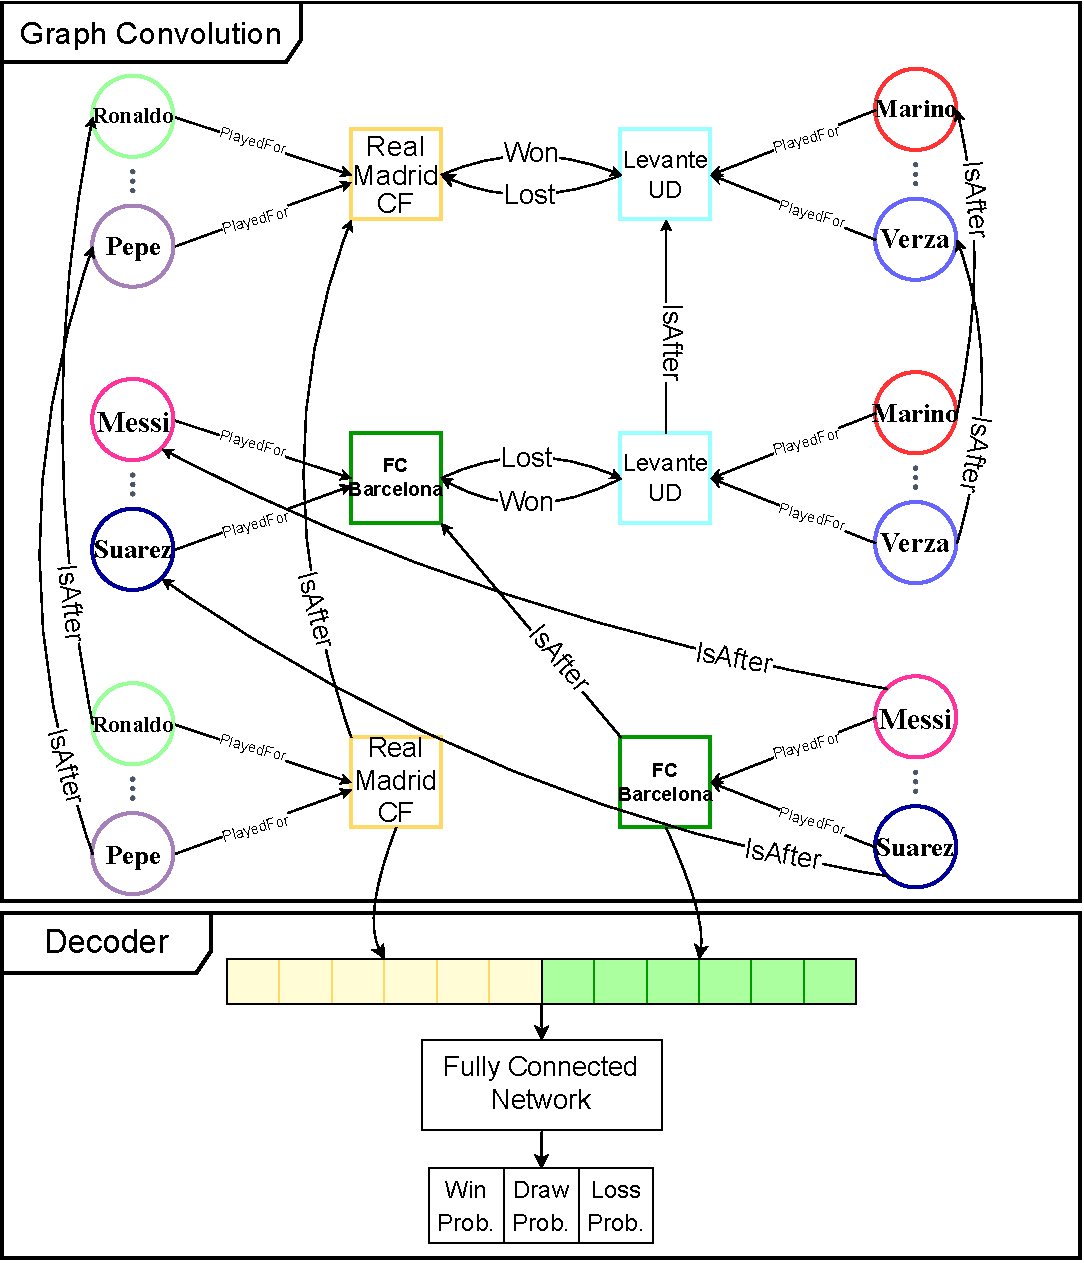
\includegraphics[width=0.40\textwidth]{GraphConv_Decoder.pdf}
         \caption{ An illustration of the proposed framework for sport result prediction.
         }
    \label{fig:model}
\end{wrapfigure}

In the next step, by applying the graph representation learning methods to the graph of the teams/players and their relations, a representation is obtained for each. Finally, the representations of the teams are used to predict the outcome of an upcoming match. An overall architecture of the introduced framework is depicted in figure \ref{fig:model}.
This approach provides several capabilities simultaneously: 

 1-Handling player learning can be achieved easily through this model, 2-There is no need for feature engineering and the learner can predict the match outcomes with raw input features (if any) and representation learning, 3-The evolution of players and teams over time becomes part of the Spatio-Temporal graph structure and does not require a separate solution, 4-The relational nature of the input data is well suited to this model. In addition, the process for adding any background information, if any, as a fact to the constructed graph is quite straightforward. 

% \begin{enumerate}
%     \item Handling player learning can be done easily through this model. 
%     \item There is no need for feature engineering and the learner can predict the match outcomes with raw input features (if any) and representation learning. 
%     \item The evolution of players and teams over time becomes part of the Spatio-Temporal graph structure and does not require a separate solution. 
%     \item 
%     The model is well-suited to the relational nature of input data on the problem of predicting the match's outcome.
%     In addition, the process for adding any background information, if any, as a fact to the constructed graph is quite straightforward.

% \end{enumerate}

\paragraph{Results} To evaluate the proposed method, we used soccer data from 9 leagues between 2008 and 2016 available at: \url{https://www.kaggle.com/hugomathien/soccer} 
The results of conducted experiments demonstrate that our framework outperforms other methods in almost all leagues in terms of accuracy and RPS metrics. Moreover, the visualization of the learnt representation of players, displayed in figure \ref{fig:playerVisualization}, illustrate that the proposed model has been able to bring players with similar abilities closer together in the latent space. This result is interesting in that our model has no information about the number of goals, passes, dribbles or any other personal information about the players. There is only one input: the results of the matches in which they participated.
To do an ablation study, we removed player nodes and player participation information from our method. 
Using our proposed method without this information, we found that the overall accuracy decreased from 50.36\% to 49.63\%, indicating that although the proposed framework still has a good ability to predict the outcome of the matches, participation information is still required.

\begin{figure}[!ht]
    \centering
    \begin{subfigure}{0.45\linewidth}
        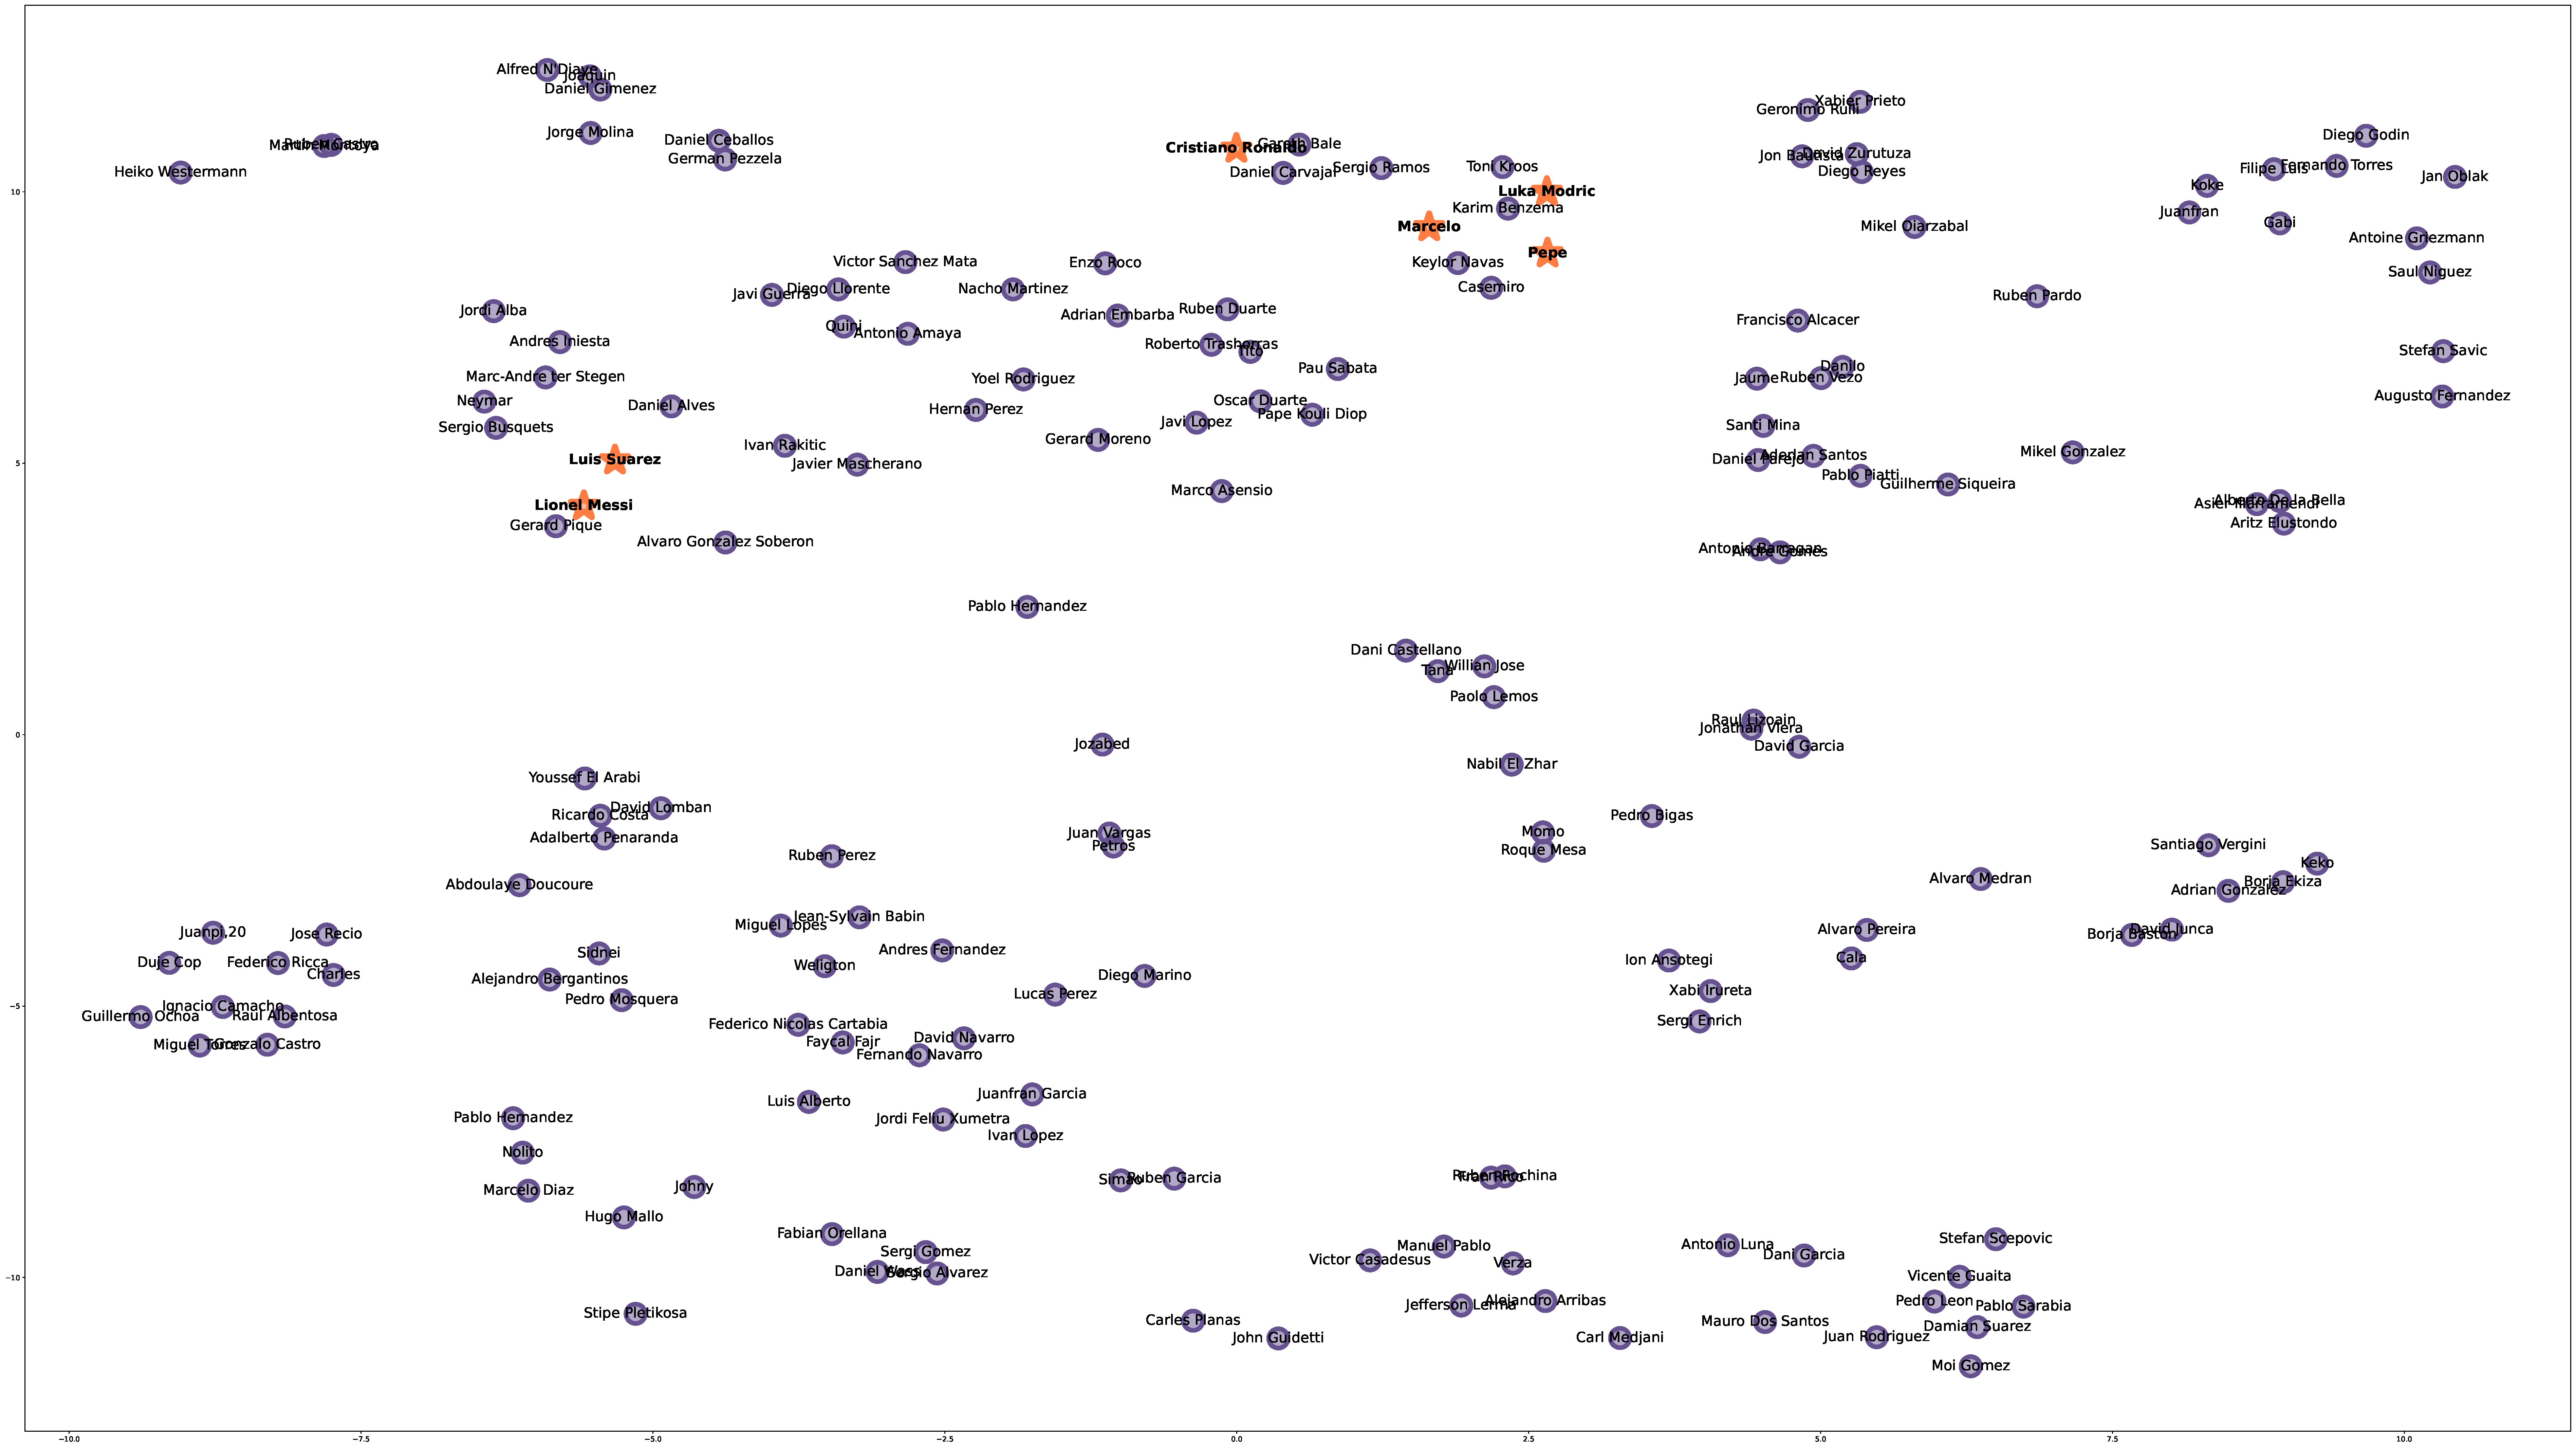
\includegraphics[width=\linewidth]{players_pretrain.pdf}
        \caption{Pre-Train Players' Representations}
    \end{subfigure}
    \begin{subfigure}{0.45\linewidth}
        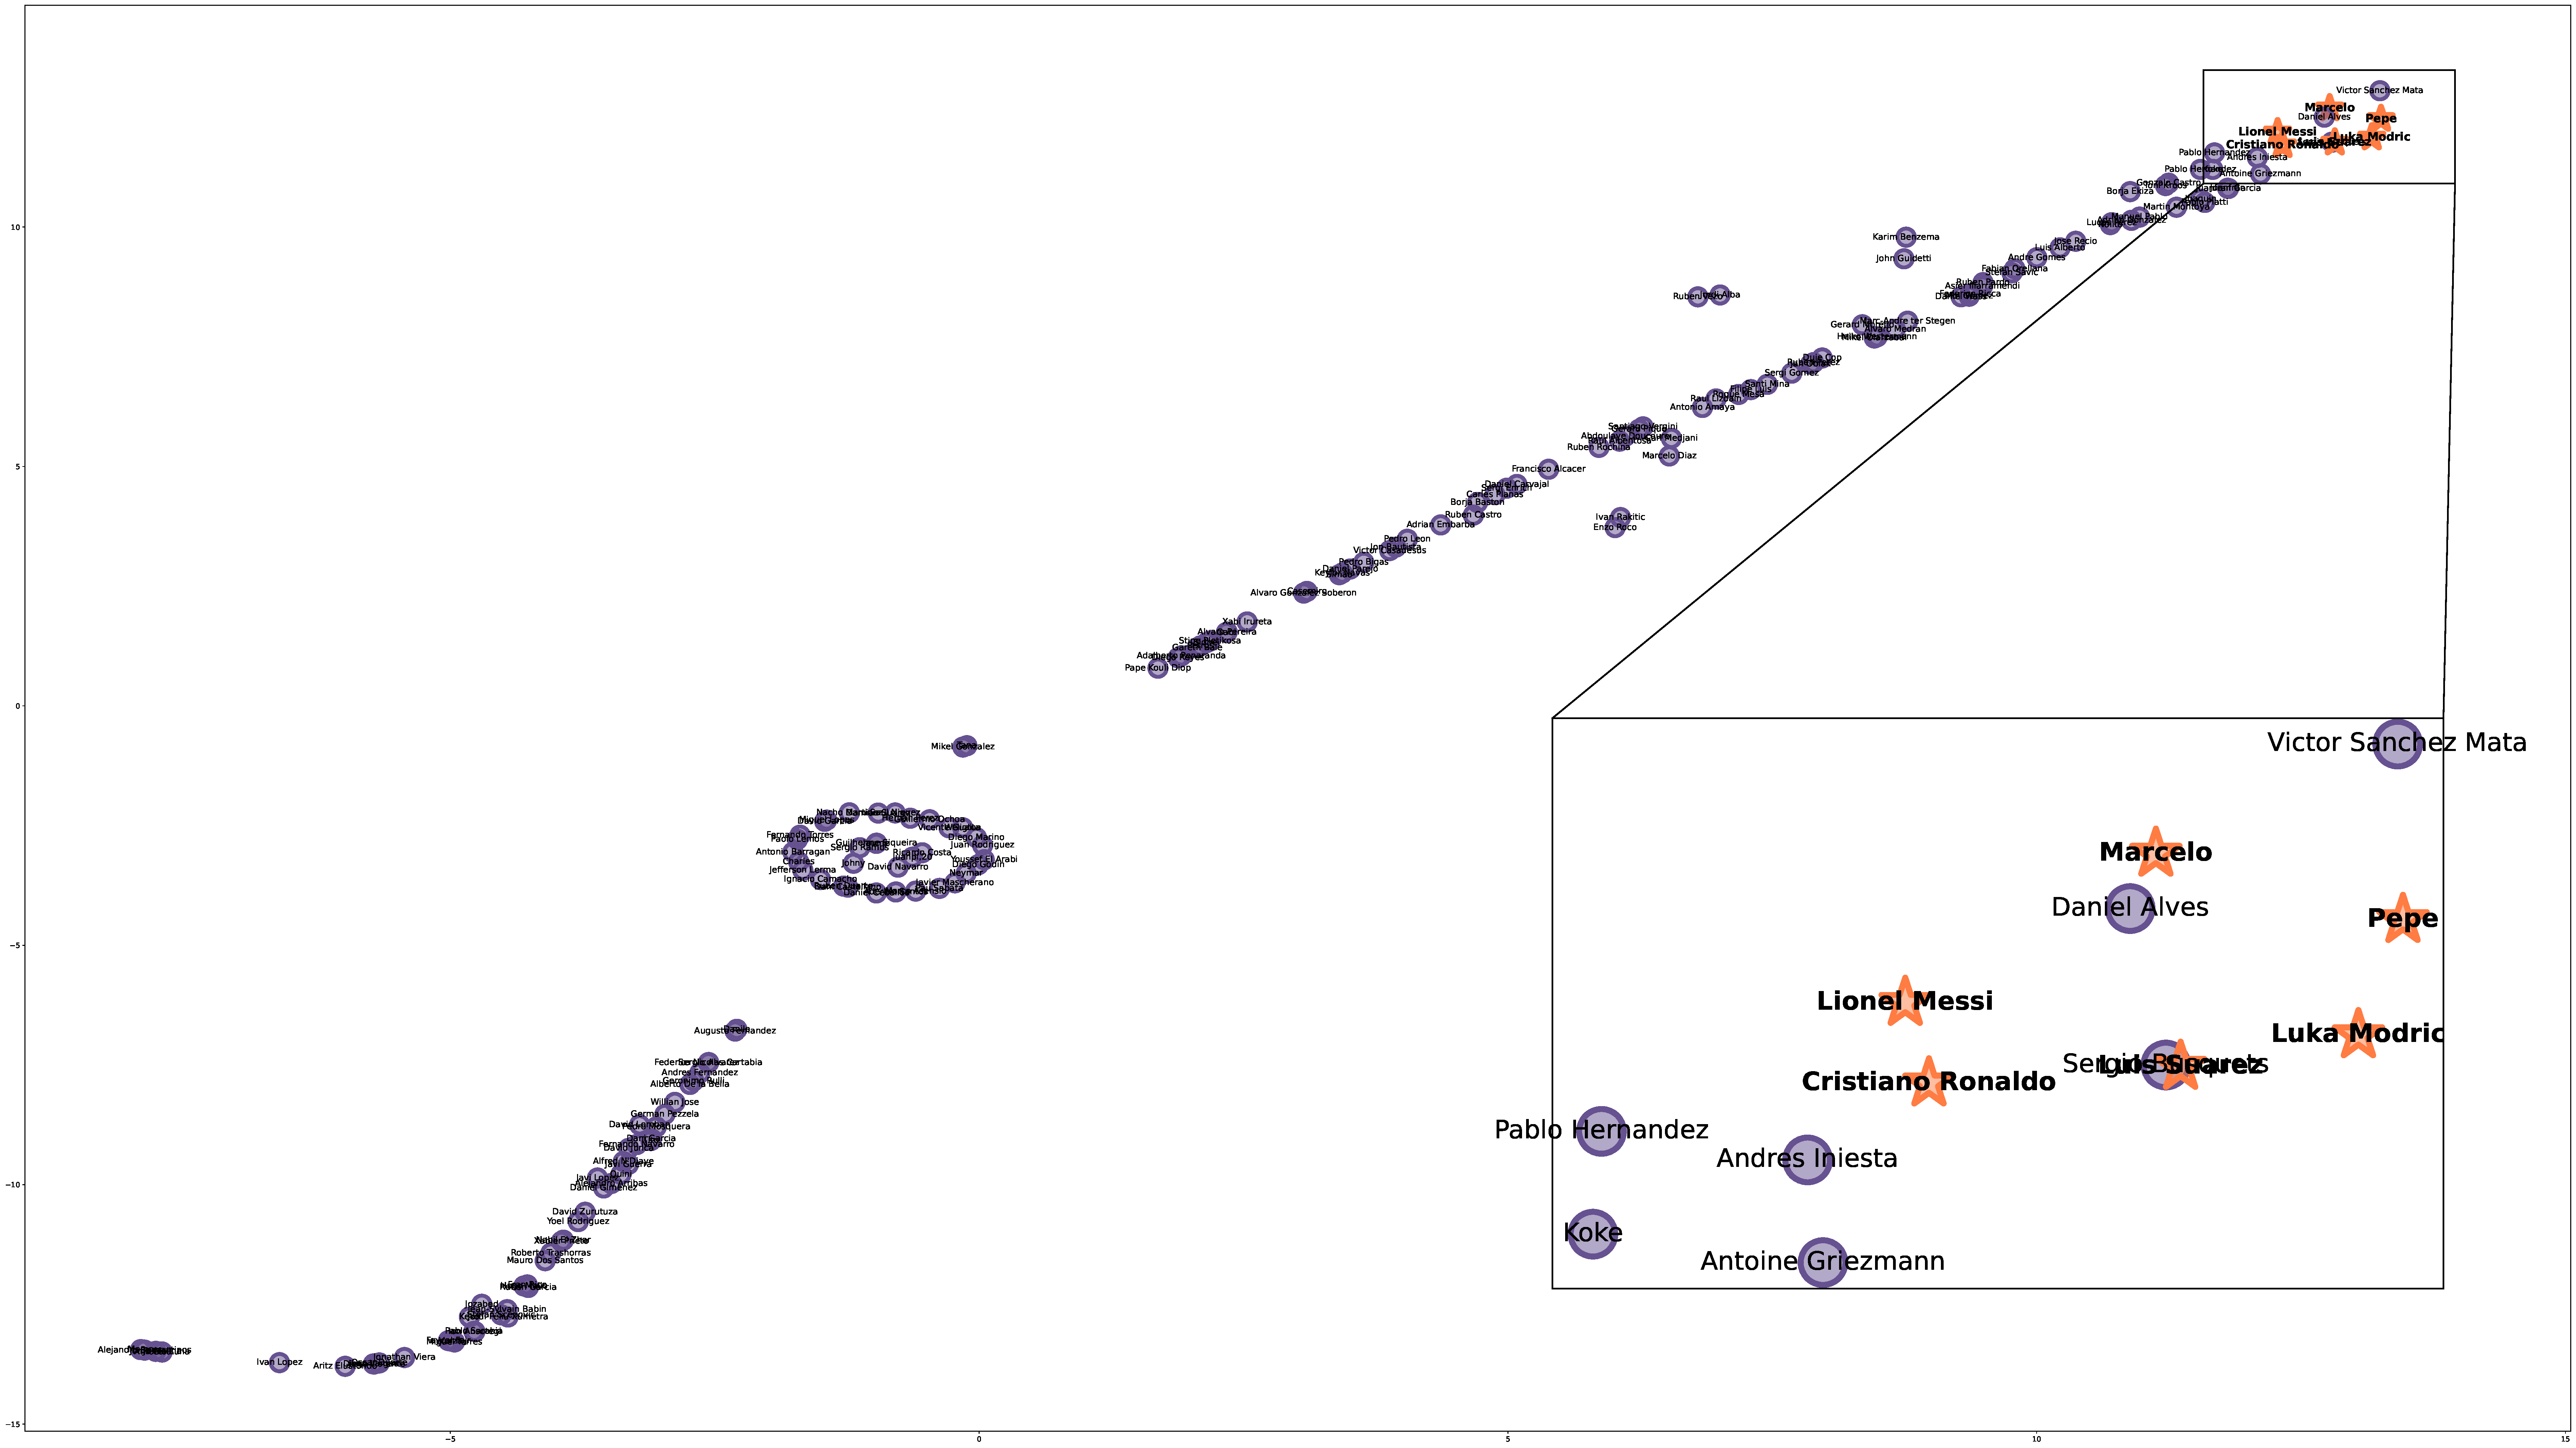
\includegraphics[width=\linewidth]{players.pdf}
        \caption{Post-Train Players' Representations}
    \end{subfigure}
 
     \caption{2D representation of the Spain LIGA BBVA 2015-2016's last match week players obtained via the Pre-Train (a) and the Post-Train (b) models.},
\label{fig:playerVisualization}
\end{figure}
\bibliographystyle{plain}
\bibliography{references}
\end{document}
